
\section{Examples}

The previous sections dealt with the main software architecture and program utilities of the UCVM framework. Here, we present a few practical examples that demonstrate how to retrieve and plot data from models registered in the framework. Space limitations prevent us from providing examples for all utilities. However, the reader can consult the General User Guide (see Table \ref{tab:manuals}) for additional examples and details, which also includes examples of how to use the UCVM API in C codes.

\subsection{Querying Velocity Models}

Querying velocity models is the most basic functionality provided by UCVM. From a terminal, this can be done simply by invoking the command-line tool \texttt{ucvm\_query} as follows.

\begin{lstlisting}[
	frame=none,
	basewidth={0.45em,0.4em},
	basicstyle=\ttfamily\footnotesize,breaklines=true,
	linewidth=0.98\columnwidth,xleftmargin=0.065\columnwidth,
	numbers=left,numberblanklines=true,numberstyle=\scriptsize\color{mylistingnclr},style=optional]
> ./ucvm_query -f $UCVM_DIR/conf/ucvm.conf -m cvms @< [input]@
\end{lstlisting}

\noindent
Here, \texttt{ucvm.conf} is a configuration file which is created at installation time and contains information about the models available in the framework as installed; the flag ``\texttt{-f}'' indicates the location of this configuration file; and the flag ``\texttt{-m}'' preceeds the label of the model from which properties are to be retrieved. The input, which may be optionally given in a file, are the longitude, latitude, and depth of the queried point. Similarly, one can also query a model for the depth of a threshold velocity using the \texttt{basin\_query} command.

\begin{lstlisting}[
	frame=none,
	basewidth={0.45em,0.4em},
	basicstyle=\ttfamily\footnotesize,breaklines=true,
	linewidth=0.98\columnwidth,xleftmargin=0.065\columnwidth,
	numbers=left,numberblanklines=true,numberstyle=\scriptsize\color{mylistingnclr}]
> ./basin_query $UCVM_DIR/conf/ucvm.conf -m cvms -v 2500
\end{lstlisting}

\noindent
In this case, the configuration file parameter requires no flag, and the flag ``\texttt{-v}'' indicates the threshold velocity in m/s.

\subsection{Creating Structured and Semi-Unstructured Meshes}

As described before, the UCVM programs \texttt{ucvm2mesh} and \texttt{ucvm2etree} can be used to create materialized velocity models in the form of regular grids or semi-unstructured meshes, respectively. These two utilities are invoked by typing:

\begin{lstlisting}[
	frame=none,
	basewidth={0.45em,0.4em},
	basicstyle=\ttfamily\footnotesize,breaklines=true,
	linewidth=0.98\columnwidth,xleftmargin=0.065\columnwidth,
	numbers=left,numberblanklines=true,numberstyle=\scriptsize\color{mylistingnclr}]
> ./ucvm2mesh -f ./ucvm2mesh.conf
\end{lstlisting}

\noindent
and

\begin{lstlisting}[
	frame=none,
	basewidth={0.45em,0.4em},
	basicstyle=\ttfamily\footnotesize,breaklines=true,
	linewidth=0.98\columnwidth,xleftmargin=0.065\columnwidth,
	numbers=left,numberblanklines=true,numberstyle=\scriptsize\color{mylistingnclr}]
> ./ucvm2etree -f ./ucvm2etree.conf
\end{lstlisting}

\noindent
Here, the \texttt{ucvm2mesh.conf} and \texttt{ucvm2etree.conf} are configuration files that specify the model(s) to be queried, the coordinates and dimensions of the regional domain to be meshed, and the projection to be used, as well as the discretization parameters (e.g., gridding size). Paths to the output binary file or etree database are also given in these configuration files. The parallel versions of these programs are invoked in similar fashion, though their configuration files require additional information about the number of processors and the domain partitioning.

\subsection{Plotting Slices and Surfaces}

UCVM comes with various plotting utilities also mentioned before: \texttt{horizontal\_slice.py}, \texttt{cross\_section.py}, \texttt{vs30.py}, \texttt{z10.py} and \texttt{z25.py}. They can all be run either interactively, by simply invoking the corresponding Python script; or directly, by passing parameters in the command line along with the program. If the latter is chosen, each value is passed on preceded by a flag that indicates the parameter correspondance. Examples with complete flag lists and parameter details are provided in the General User Guide (Table \ref{tab:manuals}). In the interactive case, on the other hand, the program is invoked without any parameters and the user is, instead, prompted for information. To illustrate the interactive process, we show next a terminal session for \texttt{horizontal\_slice.py}:

\begin{lstlisting}[
        frame=none,
        basewidth={0.45em,0.4em},
        basicstyle=\ttfamily\footnotesize,breaklines=true,
        linewidth=0.98\columnwidth,xleftmargin=0.065\columnwidth,
        numbers=left,numberblanklines=true,numberstyle=\scriptsize\color{mylistingnclr},style=input]
> @./horizontal_slice.py@
> Plot Horizontal Slice - UCVM 14.3.0
>
> This utility helps you plot a horizontal slice across the earth for one of the CVMs
> that you installed with UCVM.
>
> In order to create the plot, you must first specify the region.
>
> Please enter the bottom-left longitude from which the plot should start: @-121.5@
> Next, enter the bottom-left latitude from which the plot should start: @31@
> Enter the top-right longitude where the plot should end: @-114@
> Enter the top-right latitude where the plot should end: @38.5@
> Which grid spacing (in decimal degree units) would you like (usually, this is 0.01): @0.01@
>
> Please enter the depth, in meters, at which you would like this plot: @1000@
>
> What would you like to plot (either vp, vs, rho, or poisson): @vs@
>
> From which CVM would you like this data to come:
>	1) CVM-S4
>	2) CVM-H 11.9.1
>	3) CVM-H 11.9.1 No GTL
>	4) CVM-S4.26
>	5) 1D
>	6) Broadband Whittier Narrows 1D Model
>	7) 1D w/ Vs30 GTL
>
> Select the CVM: @4@
>
> Finally, would you like a descritized or smooth color scale
> (enter 'd' for discrete, 's' for smooth): @d@
>
> Retrieving data. Please wait...
> Data retrieved successfully.
>
> Would you like to:
>	1) Save the data
>	2) Generate a plot
>
> Select one: @2@
\end{lstlisting}

The above session plots a horizontal slice for the values of \vs{} in the model CVM-S4.26 at a depth of 1~km between longitudes --121.5\textdegree{} and --114\textdegree{}, and latitudes 31\textdegree{} and 38.5\textdegree{}, with a grid spacing of 0.01\textdegree{}. We have highlighted in blue those entries typed by the user. The result is a PNG file with the image shown in Figure~\ref{fig:hslice}. All of the other plotting scripts bundled with UCVM work in a very similar manner.


\begin{figure}%[ht!]
	\centering
	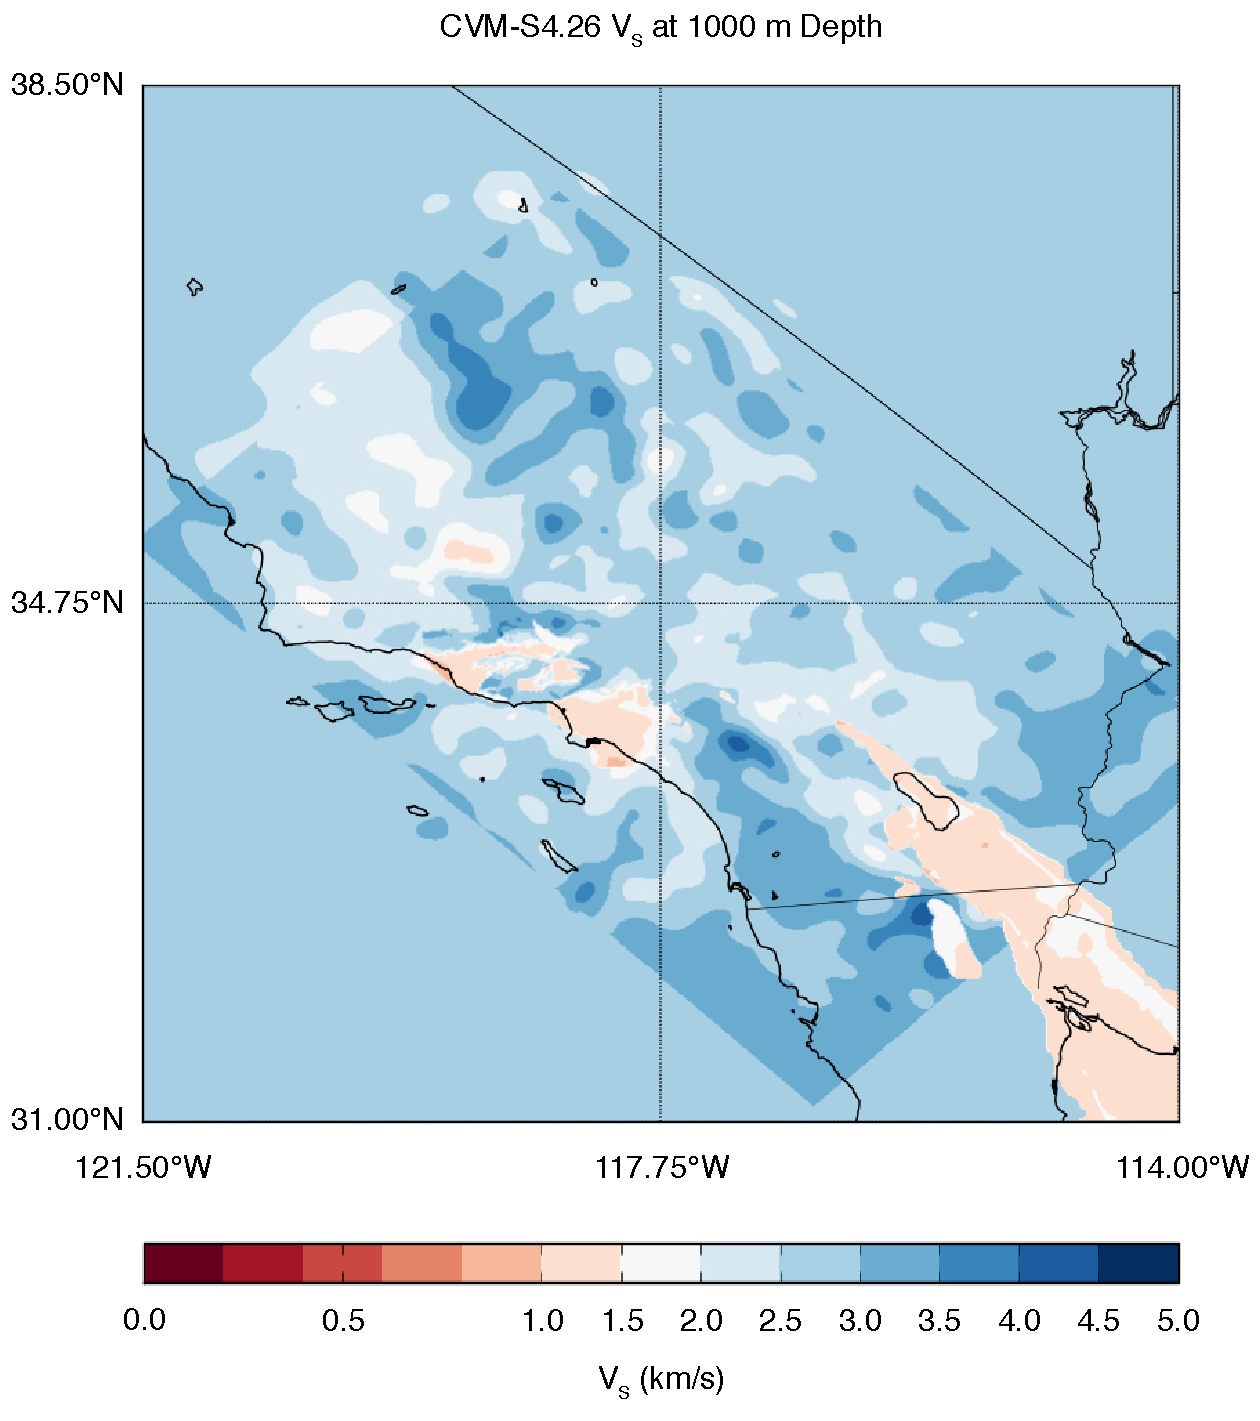
\includegraphics
		[width=\columnwidth]
		{figures/pdf/hslice}
	\caption{Example of a horizontal slice of the model CVM-S4.26 for values of \vs{} generated using the plotting utility \texttt{horizontal\_slice.py}.}
	\label{fig:hslice}
\end{figure}

